%----------------------------------------------------------------------------------------
%	PACKAGES AND OTHER DOCUMENT CONFIGURATIONS
%----------------------------------------------------------------------------------------

\documentclass{article}

\usepackage[utf8]{inputenc}
\usepackage{amssymb}
\usepackage{amsmath}
\usepackage{float}
\usepackage{latexsym}
\usepackage{subcaption}
\usepackage{gensymb}
\usepackage{caption}
\usepackage{fancyhdr} % Required for custom headers
\usepackage{lastpage} % Required to determine the last page for the footer
\usepackage{extramarks} % Required for headers and footers
\usepackage[usenames,dvipsnames]{color} % Required for custom colors
\usepackage{graphicx} % Required to insert images
\usepackage{listings} % Required for insertion of code
\usepackage{courier} % Required for the courier font
\usepackage{lipsum}
\usepackage{tabularx}
\usepackage{color}

\definecolor{mygreen}{rgb}{0,0.6,0}
\definecolor{mygray}{rgb}{0.5,0.5,0.5}
\definecolor{mymauve}{rgb}{0.58,0,0.82}

\lstset{
  backgroundcolor=\color{white},   % you must add \usepackage{color} or \usepackage{xcolor}
  breaklines=true,                 % sets automatic line breaking
  captionpos=b,                    % sets the caption-position to bottom
  commentstyle=\color{mygreen},    % comment style
  escapeinside={\%*}{*)},          % if you want to add LaTeX within your code
  extendedchars=true,              % lets you use non-ASCII characters; for 8-bits encodings only, does not work with UTF-8
  frame=single,	                   % adds a frame around the code
  keepspaces=true,                 % keeps spaces in text, useful for keeping indentation of code (possibly needs columns=flexible)
  keywordstyle=\color{blue},       % keyword style
  language=Octave,                 % the language of the code
  otherkeywords={*,...},           % if you want to add more keywords to the set
  numbers=left,                    % where to put the line-numbers; possible values are (none, left, right)
  numbersep=5pt,                   % how far the line-numbers are from the code
  numberstyle=\tiny\color{mygray}, % the style that is used for the line-numbers
  rulecolor=\color{black},         % if not set, the frame-color may be changed on line-breaks within not-black text (e.g. comments (green here))
  showspaces=false,                % show spaces everywhere adding particular underscores; it overrides 'showstringspaces'
  showstringspaces=false,          % underline spaces within strings only
  showtabs=false,                  % show tabs within strings adding particular underscores
  stepnumber=2,                    % the step between two line-numbers. If it's 1, each line will be numbered
  stringstyle=\color{mymauve},     % string literal style
  tabsize=2,	                   % sets default tabsize to 2 spaces
  title=\lstname                   % show the filename of files included with \lstinputlisting; also try caption instead of title
}

\topmargin=-0.45in
\evensidemargin=0in
\oddsidemargin=0in
\textwidth=6.5in
\textheight=9.0in
\headsep=0.25in
\linespread{1.1} % Line spacing

%\pagestyle{fancy}
\lhead{Set Header} % Top left header
\chead{}
\lfoot{\lastxmark} % Bottom left footer
\cfoot{} % Bottom center footer
\rfoot{Page\ \thepage} % Bottom right footer
\renewcommand\headrulewidth{0.4pt} % Size of the header rule
\renewcommand\footrulewidth{0.4pt} % Size of the footer rule
\setlength\parindent{16pt} % Removes all indentation from paragraphs
\setcounter{secnumdepth}{0} % Removes default section numbers
\title{
\vspace{1in}
\textmd{\textbf{Advanced Topics in Machine Learning - Assignment 3}} \\
\author{Christoffer Thrysøe - dfv107}
}
%%%%%%%%%%%%%%%%%%%%%%%%%%%%%%%%%%%%%%%%%%%%%%%%%%%%%%%%%%%%%%%%%%%%%%%%
\begin{document}
\maketitle
\pagenumbering{arabic}
\section{1. SVM and regularization}
We consider the primal optimization of the 1-norm soft margin SVM:
\begin{align}
\label{eq:opt}
\text{minimize}_{\xi,w,b} \hspace{0.2cm} &\dfrac{1}{2} \langle w,w \rangle + C \sum\limits_{i=1}^l \xi_i \\
\label{eq:const1}
\text{subject to} \hspace{0.2cm} &y_1(\langle w,\phi(x_1) \rangle +b) \geq 1-\xi_i \hspace{0.2cm} , \hspace{0.2cm} i = 1,...,l \\
\label{eq:const2}
&\xi_i \geq 0 \hspace{0.2cm} , \hspace{0.2cm} i=1,...,l
\end{align}
and we wish to prove that, when $w$, $b$ is fixed, the optimal slack variable is given by:
\begin{equation}
\xi_i = \text{max}(0,1-y_i(\langle w, \phi(x_i)\rangle +b )) = L_{hinge}(y_i,f(x_i))
\end{equation}
where the hinge loss is given by the following:
\begin{equation}
\label{eq:hinge}
L_{hinge}(y,f(x)) = \text{max}(0,1-yf(x))
\end{equation}
Given that the hyperplane is fixed in the optimization problem \eqref{eq:opt}, the only variable we are minimizing with respect to is the slack variables. Clearly the problem is minimized, when we have the smallest feasible slack variable, i.e the one which still satisfies it's constraints, listed in \eqref{eq:const1} and \eqref{eq:const2}. We note that we can re-write the constraint \eqref{eq:const1} as followed:
\begin{align}
y_1(\langle w,\phi(x_1) \rangle +b) &\geq 1-\xi_i \Rightarrow \\
\label{eq:ineq}
\xi_i &\geq 1-y_1(\langle w,\phi(x_1) \rangle +b)
\end{align}
It is clear that given the constraint in \eqref{eq:const1} and that $\xi_i \geq 0$ for all $i$, to minimize \eqref{eq:opt}, the inequality in \eqref{eq:ineq} must be an equality, because we want the smallest feasible slack variable. Thus we have:
\begin{equation}
\label{eq:mightbeneg}
\xi_i = 1-y_1(\langle w,\phi(x_1) \rangle +b)
\end{equation}
by constraint \eqref{eq:const2}, $\xi_i$ must be greater than or equal to zero. \eqref{eq:mightbeneg} will get negative for points correctly classified and above/below the margin, in this case we do not need a slack variable, thus we take the following:
\begin{equation}
\xi_i = \text{max}(0,1-y_i(\langle w, \phi(x_i)\rangle +b ))
\end{equation}
which is equal to the hinge-loss defined in \eqref{eq:hinge}, where $y$ is the target value and $(\langle w,\phi(x_1) \rangle +b)$ is the predicted value. 
\section{2. Karush-Kuhn-Tucker (KKT) theorem}
Given an optimization problem, we formulate the problem as followed:
\begin{align}
\text{minimize } &f(w) \\
\label{eq:ineqconst}
\text{subject to } &g_i(w) \leq 0 \\
&h_j(w) = 0
\end{align}
Thus an optimization problem can have multiple inequality and equality constraints. For a primal optimization problem, we define the Lagrangian function as:
\begin{equation}
L(w,\lambda,\mu) = f(w) + \sum_{i=1}^m \lambda_i h_i(w) + \sum\limits_{i=1}^k \mu_i g_i(w)
\end{equation}
Then if the following Karush-Kuhn-Tucker conditions are satisfied, we have that $w^*$ is a a global minimum, if we can find values for $\lambda^*$ and $\mu^*$ such that the following conditions are satisfied:
\begin{align}
\dfrac{\partial L (w^*, \lambda^*, \mu^*)}{\partial w} &= 0 \\
\dfrac{\partial L (w^*, \lambda^*,\mu^*)}{\partial \lambda} &= 0 \\
\mu_i^* g_i(w^*) &= 0 \\
g_i(w^*) &\leq 0 \\
\mu_i^* &\geq 0
\end{align}
for all $i=1,..,k$ \\
Note that for the following problems, instead of minimizing $||w||$, I will be minimizing $||w||^2$ as written on the discussion forum.
\subsection{1}
\begin{align}
\text{minimize } &||w||^2 \\
\text{subject to } &w_1 + w_2 + 1 \geq 0
\end{align}
First the inequality is rephrased to the same form of \eqref{eq:ineqconst}, thus the constraint is as followed:
\begin{equation}
g(w) = -w_1 - w_2 -1 \leq 0
\end{equation}
writing up the Lagrangian function we get:
\begin{align}
L(w,\mu) &= ||w||^2 + \mu(-w_1 - w_2 - 1) \\
\label{eq:optprob1}
&= \sqrt{w_1^2 + w_2^2}^2 + \mu(-w_1 - w_2 - 1)
\end{align}
note that we don't include the $\lambda$ term, because we only have an equality constraint. Taking the derivative of \eqref{eq:optprob1} with respect to $w_1$ and $w_2$, and setting them to zero we get:
\begin{align}
\label{eq:deriv1}
\dfrac{\partial L (w, \mu)}{\partial w_1} &= 2 w_1 - \mu = 0 \\
\label{eq:deriv2}
\dfrac{\partial L (w, \mu)}{\partial w_2} &= 2 w_2 - \mu = 0
\end{align}
for the two derivatives, shown in \eqref{eq:deriv1} and \eqref{eq:deriv2}, we note that $w_1$ and $w_2$ must be equal, otherwise the two equations don't hold. We also note that they must not be negative as otherwise we would break the condition of $\mu \geq 0$ If we have that $w_1=w_2=0$ then the above would hold for $\mu = 0$. If we check the KKT conditions we have:
\begin{align}
\dfrac{\partial L (w^*, \mu^*)}{\partial w_1} &= 2 w_1 - \mu^*
 = 2 \times 0 - 0 = 0 \\
\dfrac{\partial L (w^*, \mu^*)}{\partial w_2} &= 
2 w_2 - \mu^* = 2 \times 0 - 0 = 0 \\
\mu^* g(w^*) &= \mu^* (-w_1 - w_2 -1) = 0 (0 - 0 - 1) = 0 \\
g(w^*) &= (-w_1 - w_2 - 1) = (0 - 0 - 1) = -1 \leq 0 \\
\mu^* &= 0 \geq 0
\end{align}
Thus all conditions are satisfied and we have that $w^* = (0,0)$ is a solution to the minimization.
\subsection{2}
\begin{align}
\text{minimize } &||w||^2 \\
\text{subject to } &w_1 + w_2 + 1 \leq 0
\end{align}
We have the following Lagrangian function:
\begin{equation}
L(w,\mu) = \sqrt{w_1^2 + w_2^2}^2 + \mu(w_1 + w_2 + 1)
\end{equation}
The derivative, with respect to $w$, is given by:
\begin{align}
\label{eq:deriv3}
\dfrac{\partial L (w, \mu)}{\partial w_1} &= 2 w_1 + \mu = 0 \\
\label{eq:deriv4}
\dfrac{\partial L (w, \mu)}{\partial w_2} &= 2 w_2 +\mu = 0
\end{align}
We can easily identify that the constraint is satisfied when $w_1 = w_2 = -0.5$. If we use this value of $w$ in \eqref{eq:deriv3} and \eqref{eq:deriv4} we get that $\mu = 1$ and therefore:
\begin{equation}
2 \times -0.5 + 1 = 0 
\end{equation}
We have shown that:
\begin{equation}
\dfrac{\partial L (w^*, \mu^*)}{\partial w} = 0
\end{equation}
now we wish to show that the rest of the KKT conditions are satisfied as well:
\begin{align}
\mu^* g(w^*) &= \mu^* (w_1 + w_2 + 1) = 1 (-0.5 +(-0.5) + 1) = 0 \\
g(w^*) &= (w_1 + w_2 + 1) = (-0.5 + (-0.5) + 1) = 0 \leq 0 \\
\mu^* &= 1 \geq 0
\end{align}
Thus all conditions are satisfied and we have that $w^* = (-0.5,-0.5)$ is a solution to the minimization problem.
\subsection{3}
\begin{align}
\text{minimize } &||w||^2 \\
\label{eq:lastcons}
\text{subject to } &2w_1 + 2w_2 + 2 = 0
\end{align}
We have the following Lagrangian function:
\begin{equation}
\label{eq:lambd}
L(w,\mu) = \sqrt{w_1^2 + w_2^2}^2 + \lambda(2w_1 + 2w_2 + 2)
\end{equation}
Taking the derivative of \eqref{eq:lambd} with respect to $w_1$ and $w_2$, and setting them to zero we get:
\begin{align}
\label{eq:deriv5}
\dfrac{\partial L (w, \mu)}{\partial w_1} &= 2 w_1 + 2 \lambda = 0 \\
\label{eq:deriv6}
\dfrac{\partial L (w, \mu)}{\partial w_2} &= 2 w_1 + 2 \lambda = 0
\end{align}
we note again that the above is only satisfied when $w_1 = w_2$. The constraint in \eqref{eq:lastcons} is satisfied when $w_1 = w_2 = -0.5$.
From \eqref{eq:deriv5} we set $w_1=w_2=-0.5$ and solve for $\lambda$:
\begin{align}
2 \times -0.5 + \lambda &= 0 \Rightarrow \lambda = 0.5
\end{align}
To prove that the KKT conditions are satisfied we also need to prove that:
\begin{equation}
\dfrac{\partial L (w^*, \lambda^*)}{\partial \lambda} = 0
\end{equation}
Taking the derivative of \eqref{eq:lambd} with respect to $\lambda$ and inputting the value for $w$ we get:
\begin{align}
\dfrac{\partial L (w^*, \lambda^*)}{\partial \lambda} &= 2w_1 + 2w_2 + 2 = 2\times -0.5 + 2 \times -0.5 + 2 = 0
\end{align}
Thus all conditions are satisfied and we have that $w^* = (-0.5,-0.5)$ is a solution to the minimization problem.
%\section{3. SVM model selection}
%For the Gaussian kernel, the parameter $\gamma$ controls the width of the kernel. For larger values of $\gamma$ the kernel is smooth and the geometry of the transformed feature space will also be smooth. A small $\gamma$ results in a narrow kernel and the feature space will have more contrast. Choosing a narrow kernel will most likely lead to over-fitting as the geometric surface of the transformed feature space allows for a greater deal of separation of the data. The parameter $C$ is the regularization parameter and controls the penalty we add to the slack variables. A large value of $C$ means that we allow more slack variables and thus can obtain a larger margin, whereas a large value for $C$ will penalize slack variable, which will cause the SVM
%to classify as many data points as possible, often resulting in a smaller margin and thus a worse generalization. \\
%When performing grid-search to find the optimal parameters for $\gamma$ and $C$ over cross validation, 
\section{3. PAC-Bayesian Aggregation}
For this assignment, I have used the Support Vector Machine library LibSVM \cite{svm}. First I will describe how the baseline was implemented, and then how the experiment from \cite{article} was performed. The implementation of the baseline is given in the file \texttt{crossValidate.py}, the experiment is implemented in the file \texttt{experiment.py} and the plotting is given in the file \texttt{plotgraph.py}. \\ For the baseline, the Ionosphere data \cite{data} was first loaded and the target values was converted such that:
\begin{equation}
y_i = \begin{cases}
1 &\text{if $y_i = b$}\\
-1 &\text{if $y_i = g$}
\end{cases}
\end{equation}
The data was then randomly partitioned into a training and test set, where the training set contains 225 observations, and the test set contains 126 observations. This division follows the one used in \cite{article}. For both parts of the assignment, the RBF-kernel SVM is used. To find appropriate values for the RBF-kernel bandwidth parameter $\gamma$, the Jaakkola heuristic was implemented. This was done by taking the distance for each training example to the rest of the training examples. These distances was sorted in ascending order. The closest training example, with a different target label, was then located, and it's distance to the training point was added to a list $G$. Thus index $i$ in $G$ is defined as:
\begin{equation}
G(x_i) = \text{min}_{(X_j,Y_j)\in S \wedge Y_i \neq Y_j} ||X_i - X_j||
\end{equation}
the median of $G$ was then taken and the Jaakkola seed was defined by:
\begin{equation}
\gamma_J = \dfrac{1}{2 \cdot \text{ median}(G)^2}
\end{equation}
Getting $\gamma_J$ on the entire data (that is training and test) the following Jaakkola seed was achieved:
\begin{equation}
\gamma_J = 0.14349
\end{equation}
(The $\gamma_J$ used for the baseline is determined solely on the training data, i.e. no access to the test data).
The $\gamma$ and $C$ values, used for training the Support Vector Machine was then defined as:
\begin{align}
\gamma &\in \lbrace y_J \cdot 10^i | i \in \lbrace -4,-3,-2,-1,0,1,2,3,4 \rbrace \rbrace  \\
C &\in \lbrace 10^{-3}, 10^{-2}, 10^{-1}, 10^0, 10^1, 10^2, 10^3 \rbrace
\end{align}
Grid search was then performed using 5-fold cross validation, to find optimal hyper parameters. For each value of $C$ and $\gamma$, the training set was randomly split into 5 equal sized sets. For each round of the cross validation, the SVM was trained on the four partitions combined, where the fifth partition was used as a validation set. The average error over these five validation sets was then taken. The choosing of $C$ and $\gamma$, which resulted in the lowest average error over the five validation sets, was used as final hyper parameters. The found hyper parameters was then used for training of the SVM on the entire training set. This trained model was then used to get the test error on the test set. Running the baseline 30 times, the following hyper parameters was found:
\begin{align*}
C &= 10^1 = 10 \\
\gamma &= \gamma_J \cdot 10^0 = \gamma_J
\end{align*}
The following table shows the average training ($\hat{L}(h,S)$) and test ($L(h)$) errors and their standard deviation over the 30 runs:
\begin{table}[H]
\centering
\caption{Average training and test errors over 10 runs and their standard deviation.}
    \begin{tabular}{|c|c|c|c|}
        \hline
        $\hat{L}(h,s)$ & $L(h)$ & $\sigma_{\hat{L}(h,s)}$ & $\sigma_{L(h)}$ \\ \hline
        0.0192 & 0.0577 & 0.0140  & 0.0171 \\ \hline
    \end{tabular}
\end{table}
The average running time of the baseline was:
\begin{equation}
t_{baseline} = 2,87 \text{ sec}
\end{equation}
The running time included the cross validation, hyper parameter selection, the training of the final model and the applying of the model on the unseen test data to get the test error. \\ \\
The experient was done as followed. First a training and test set was created, following the same partition size as for the baseline. Given a number of $m$ subsets, each subset was assigned $d+1=r$ random points from the training data. The remaining $n-r$ points was used as a validation set, where $n$ is the length of the training data. Each $m$ subsets, containing $35$ points each, was then used for training an SVM, where the validation set, containing $n-r$ points each, was used for validation of the weak classifier. The bandwidth parameter $\gamma$ of the RBF-kernel was randomly selected from the same list of $\gamma$ as used in the baseline. For the value of $C$ \cite{article} notes that setting $C$ was not necessary as the hyperplane was able to perfectly separate the $35$ training points. I did however experience that setting $C$ was necessary in order to correctly classify the 35 training points, this setting of $C$ however did not influence the final result of the classifier. Once the validation error was achieved for each $m$ subsets, the distribution $\rho$ was found using alternating minimization of the following bound, which holds with probability greater than $1- \delta$:
\begin{equation}
\label{eq:bound}
\mathbb{E}_\rho[L(h)] \leq \dfrac{\mathbb{E}_\rho [\hat{L}^{val}(h,S)]}{1- \frac{\lambda}{2}}+ \dfrac{KL(\rho || \pi) + \text{ ln } \frac{(n-r)+1}{\delta}}{\lambda(1-\frac{\lambda}{2})(n-r)}
\end{equation}
where $\lambda \in (0,2)$.
The alternating minimizations consist of alternating minimizing $\rho$ and $\lambda$. The update rule for $\rho$ is defined as:
\begin{equation}
\label{eq:min1}
\rho(h) = \dfrac{ \pi(h)e^{-\lambda(n-r) (\hat{L}^{val}(h,S)- \hat{L}^{val}_{\text{min}})}}{\sum_{h'} \pi(h') e^{-\lambda(n-r) (\hat{L}^{val}(h,S) - \hat{L}^{val}_{\text{min}})} }
\end{equation}
The update rule for $\lambda$ is defined as followed in Yevgeny's lecture notes (equation 3.15):
\begin{align}
\lambda = \dfrac{2}{ \sqrt{ \dfrac{2n \mathbb{E}\rho \left[\hat{L}(h,S)\right]}{ \text{KL}(\rho || \pi) + \text{ ln }\dfrac{n+1}{\delta}} +1 } +1}
\end{align}
The update term can be re-written to suit our validation error, and use the definition of $KL(\rho || \pi)$ from the lecture notes:
\begin{align}
\lambda &= \dfrac{2}{ \sqrt{ \dfrac{2(n-r) \mathbb{E}\rho \left[\hat{L}^{val}(h,S)\right]}{ \text{KL}(\rho || \pi) + \text{ ln }\dfrac{(n-r)+1}{\delta}} +1 } +1}\\
&= \dfrac{2}{ \sqrt{ \dfrac{2(n-r) \mathbb{E}\rho \left[\hat{L}^{val}(h,S)\right]}{ \mathbb{E}_\rho\left[ \text{ln}  \dfrac{1}{\pi} \right] - H(\rho) + \text{ ln }\dfrac{(n-r)+1}{\delta}} +1 } +1}\\
\label{eq:min2}
&= \dfrac{2}{ \sqrt{ \dfrac{2(n-r) \left( \sum\limits_{h \in \mathcal{H}} \rho(h) \hat{L}^{val}(h,S)\right)}{ \left( \sum\limits_{h \in \mathcal{H}}  \rho(h)  \text{ln}  \dfrac{1}{\pi} \right) - \left( - \sum\limits_{h \in \mathcal{H}} \rho(h) \text{ ln } \rho(h) \right) + \text{ ln }\dfrac{(n-r)+1}{\delta}} +1 } +1}
\end{align}
Where in both terms, the prior distribution $\pi$ was chosen to be uniform, that is $\pi(h) = 1/m$. The alternating minimization was performed, by initially setting $\lambda = 2.0$ and then finding the distribution $\rho$ from \eqref{eq:min1}, using this obtained value for $\rho$ to find $\lambda$ from \eqref{eq:min2}. This alternating minimization was performed until the change in the norm of $\rho$ (treated as a list for each $\rho(h)$) was below a threshold $\epsilon$ and the change in the parameter $\lambda$ was below a threshold $\epsilon$, where for both stopping criteria $\epsilon = 2.224 \cdot 10^{-16}$. For the minimization we had $\delta = 0.05$. The obtained distribution $\rho$ minimizing the bound in \eqref{eq:bound} was then used to perform $\rho$-weighted majority vote, which is defined as followed:
\begin{equation}
\label{eq:majority}
MV_\rho(X) = \text{sign}\sum\limits_{h \in \mathcal{H}} \rho(h) h(X)
\end{equation}
where each $h$ is the SVM model, trained on the random $r$ points, used for getting the validation errors. The majority vote was used on the yet unseen test data to get the test error. The bound from theorem 3.13 from Yevginev's lecure notes, which we would like to plot is defined as:
\begin{equation}
\label{eq:bound1}
\text{kl} \left(\mathbb{E}_\rho\left[ \hat{L}^{val}(h,S) \right] ||  \mathbb{E}_\rho\left[ L(h) \right] \right) \geq \dfrac{ \text{KL}(\rho || \pi) + \text{ln}\dfrac{(n-r)+1}{\delta} }{n-r}
\end{equation}
To get a bound on the expected loss $\mathbb{E}_\rho\left[ L(h) \right]$, the kl divergence from \eqref{eq:bound1} was inverted numerically, taking the upper inverse. To take the upper inverse, we must solve the following:
\begin{equation}
kl^{-1^+}(\hat{p},z) = \text{max} \lbrace p : kl(\hat{p}||p) \leq z \rbrace
\end{equation}
giving the following bound, which holds with probability greater than $1-\delta$:
\begin{equation}
p \leq \text{max} \left\lbrace p: p \text{ ln} \frac{\hat{p}}{p} + (1-\hat{p}) \text{ ln } \dfrac{1-\hat{p}}{p} \leq z \right\rbrace
\end{equation}
where $\hat{p} = \sum\limits_{h \in \mathcal{H}} \rho(h) \hat{L^{val}}(h,S)$, $p = \mathbb{E}_\rho[L(h)]$ and z is defined as:
\begin{align}
z &= \dfrac{KL(\rho||\pi) + \text{ln} \dfrac{(n-r)+1}{\delta}}{n-r} \\
&= \dfrac{  \left( \sum\limits_{h \in \mathcal{H}}  \rho(h)  \text{ln}  \dfrac{1}{\pi} \right) - \left( - \sum\limits_{h \in \mathcal{H}} \rho(h) \text{ ln } \rho(h) \right) + \text{ln}\dfrac{(n-r)+1}{\delta}}{n-r}
\end{align}
The kl inequality was inverted numerically using a binary search. \\
The above was performed for 20 different values of $m$ from [1,200]. As with the baseline, for each choosing of $m$, the experiment was performed 30 times, where it's average error, bound, running time and standard deviation was taken. The running time of the Pac-Baysian aggregation included training the $m$ subsets, getting the validation error, applying alternating minimization and performing $\rho$-weighted majority vote to get the test error. Below, the error and standard deviation is listed for some of the values for $m$ (the error for all $m$ is shown in the figure):
\begin{table}[H]
\centering
\caption{The test error and standard deviation shown for some values of $m$ using Pac-Baysian Aggregation}
\label{tab:2}
    \begin{tabular}{|c|c|c|c|c|c|c|c|c|c|c|}
        \hline
      $m$  & 10 & 30 & 50 & 70 & 90 & 110 & 130 & 150 & 170 & 190
         \\ \hline
       $L(h)$ & 0.115 & 0.089 & 0.080 & 0.078 & 0.079 & 0.071 & 0.075 & 0.072 & 0.074 & 0.073 \\ \hline
$\sigma_{\text{Pac-bayes}}$  & 0.038 & 0.035 & 0.025 & 0.022 & 0.023 & 0.025 & 0.022 & 0.021 & 0.026 & 0.023  \\ \hline
    \end{tabular}
\end{table}
As evident from table \ref{tab:2} the error is decreasing and almost as low as the baseline for high values of $m$. It is also clear that the standard deviation in the results are higher than for the baseline. Figure \ref{fig:1} shows the baseline average error and time, it also shows the average error obtained from the Pac-Bayesian Aggregation, it's bound and the running as a function of the number of subsets $m$. The reported error is the zero-one loss, and the time is plotted as $seconds/10$. It is clear that when the number of subsets increases the error goes down, however the running time goes up, so there is a trade-off in achieving a low error and a reasonable running time. Interestingly for the Pac-Baysian aggregation, we are able to achieve a somewhat low error, while maintaining a very low running time. The baseline has the lowest error, but also the largest running time. As $m$ increases, the error goes towards the baseline and the running time also approaches the baseline running time.
\begin{figure}[H]
 \centering
  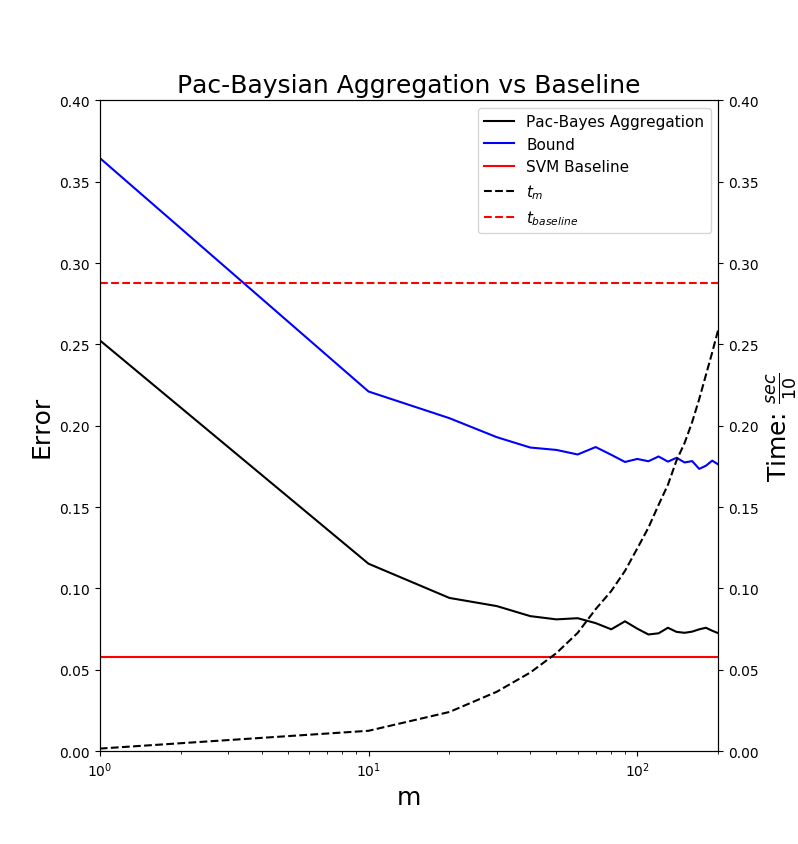
\includegraphics[width=17cm]{fig/2.png}
  \caption{\footnotesize The Pac-Baysian aggregation compared to an RBF kernel SVM tuned by cross-validation. The left y axis shows the zero-one loss, where the right axis shows the time in $sec/10$. The x axis shows the number of subsets used in the Pac-Baysian aggregation.}
\label{fig:1} 
\end{figure}

\newpage
\begin{thebibliography}{9}
\bibitem{svm}
Chih-Chung Chang and Chih-Jen Lin,  \textit{LIBSVM -- A Library for Support Vector Machines} https://www.csie.ntu.edu.tw/~cjlin/libsvm/
\bibitem{article}
Niklas Thiemann, Christian Igel, Olivier Wintenberger, and Yevgeny Seldin. \textit{A strongly quasiconvex
PAC-Bayesian bound}. In Proceedings of the International Conference on Algorithmic Learning Theory
(ALT), 2017. http://arxiv.org/abs/1608.05610.
\bibitem{data}
Arthur Asuncion and David J. Newman. UCI machine learning repository, 2007. http://archive.ics.uci.edu/ml/index.php.
\end{thebibliography}
\end{document}
